\documentclass[aspectratio=169,14pt]{beamer}
\usetheme{default}
\usepackage{fontspec}
\setmainfont{texgyrepagella-regular.otf}[BoldFont=texgyrepagella-bold.otf,ItalicFont=texgyrepagella-italic.otf,BoldItalicFont=texgyrepagella-bolditalic.otf]
\setsansfont{texgyreheros-regular.otf}[BoldFont=texgyreheros-bold.otf,ItalicFont=texgyreheros-italic.otf,BoldItalicFont=texgyreheros-bold.otf,BoldItalicFeatures={FakeSlant=0.2}]
\setmonofont{lmmono10-regular.otf}[Scale=0.85]
\setbeamertemplate{navigation symbols}{}
\usepackage{pgfpages}
\newif\ifpresenter
\ifdefined\PresenterVersion\presentertrue\else\presenterfalse\fi
\ifpresenter
  \setbeameroption{show notes on second screen=right}
  \setbeamertemplate{note page}[plain]
\fi
\usepackage{amsmath,amssymb,bm,booktabs,array,graphicx,xcolor}
\usepackage{tikz,pgfplots,adjustbox,listings,xurl}
\pgfplotsset{compat=1.18}
\usetikzlibrary{arrows.meta,positioning,calc,fit,shapes.geometric,decorations.pathreplacing,patterns}
% UIUC official brand colors, verified 2026-10-23.
% https://brand.illinois.edu/visual-identity/color
\definecolor{IlliniOrange}{HTML}{FF5F05}
\definecolor{IlliniBlue}{HTML}{13294B}
\definecolor{Storm}{HTML}{707372}
\definecolor{LightStorm}{HTML}{C6C7C6}
\definecolor{Industrial}{HTML}{1D58A7}
\definecolor{Patina}{HTML}{007E8E}
\tikzset{>=Stealth, every node/.style={font=\small,text=IlliniBlue}, box/.style={draw=IlliniBlue,rounded corners=2pt,align=center,inner sep=6pt,execute at begin node=\hyphenpenalty10000\relax}, orangebox/.style={box,draw=IlliniOrange,very thick}, edge/.style={->,thick,IlliniBlue}, accent/.style={->,very thick,IlliniOrange}}
\pgfplotsset{every axis/.append style={width=13.5cm,height=6.5cm,axis line style={IlliniBlue},tick label style={font=\small,text=IlliniBlue},label style={font=\small,text=IlliniBlue},legend style={font=\small,draw=none,fill=white},grid style={LightStorm},major grid style={LightStorm},axis lines=left,clip=false}, every axis plot/.append style={thick}}

\definecolor{slidepaper}{RGB}{234,220,201}
\setbeamercolor{background canvas}{bg=slidepaper}
\setbeamercolor{normal text}{fg=IlliniBlue}
\setbeamercolor{frametitle}{fg=IlliniBlue}
\setbeamercolor{title}{fg=IlliniBlue}
\setbeamercolor{item}{fg=IlliniOrange}
\setbeamerfont{frametitle}{size=\large,series=\bfseries}
\setbeamerfont{title}{size=\Large,series=\bfseries}
\setbeamertemplate{itemize item}{\color{IlliniOrange}$\bullet$}
\setbeamertemplate{itemize subitem}{\color{IlliniOrange}\footnotesize$\circ$}
\setbeamercolor{orangerule}{bg=IlliniOrange}
\setbeamertemplate{headline}{\begin{beamercolorbox}[wd=\paperwidth,ht=0.1cm,dp=0.1cm]{orangerule}\end{beamercolorbox}}
\setbeamertemplate{footline}{\begin{beamercolorbox}[wd=\paperwidth,ht=0.1cm,dp=0.1cm]{orangerule}\end{beamercolorbox}}
\setbeamersize{text margin left=0.65cm,text margin right=0.65cm}
\setlength{\leftmargini}{1.1em}
\newenvironment{slidebullets}{\begin{itemize}\setlength\itemsep{0.8em}}{\end{itemize}}
\pgfplotsset{every axis/.append style={legend style={fill=slidepaper}}}
\lstdefinelanguage{CoursePython}{keywords={from,import,for,in,if,else,def,return,assert,True,False,None},sensitive=true,morecomment=[l]{\#},morestring=[b]',morestring=[b]"}
\lstset{language=CoursePython,basicstyle=\ttfamily\small,keywordstyle=\color{IlliniBlue}\bfseries,commentstyle=\color{Storm},stringstyle=\color{IlliniBlue},showstringspaces=false,breaklines=true,columns=fullflexible,keepspaces=true,frame=none,aboveskip=0.7em,belowskip=0.7em}
\newcommand{\E}{\mathbb E}
\newcommand{\Var}{\operatorname{Var}}
\newcommand{\Cov}{\operatorname{Cov}}
\hypersetup{colorlinks=true,urlcolor=IlliniBlue,linkcolor=IlliniBlue}

\title{Marketing Analytics}
\subtitle{Conjoint and Product Design}
\author{By Nathan Yang}
\date{Session 05}
\begin{document}
\begin{frame}
\titlepage
\end{frame}
\begin{frame}[plain]
\begin{tikzpicture}[remember picture,overlay]
\node[inner sep=0pt] at (current page.center) {
\includegraphics[width=\paperwidth,height=\paperheight,keepaspectratio]{assets/product_choices.png}};
\end{tikzpicture}
\note{Product design changes a choice set. Sales of a new bundle can replace purchases of existing bundles or attract customers who previously chose the outside option.

Original conceptual illustration. 05\_Slides/assets/PROVENANCE.md.}
\end{frame}
\begin{frame}{A Subscription-Bundle Decision}
\usebeamercolor[fg]{normal text}
\vfill
\begin{slidebullets}
\item A firm can change quality, delivery, and monthly price.
\item Customers must trade off feasible attribute combinations.
\item The choice set includes the option to buy nothing.
\end{slidebullets}
\vfill
\note{A forced choice among paid plans estimates conditional preference. It supplies no direct category-participation margin when customers cannot opt out.

M4, Section 4.1, Marketing Analytics Lecture Notes. \url{../06_Lecture_Notes/modules/M04_Conjoint_Segmentation_and_CLV.md}}
\end{frame}
\begin{frame}{Choice-Task Design}
\usebeamercolor[fg]{normal text}
\vfill
\begin{slidebullets}
\item Vary price independently of features where feasible.
\item Use realistic combinations and clear descriptions.
\item Retain respondent identity across repeated tasks.
\end{slidebullets}
\vfill
\note{Perfect correlation between price and quality prevents their separate interpretation. Repeated answers from one person are dependent, affecting estimation and validation.

M4, Section 4.1, Marketing Analytics Lecture Notes. \url{../06_Lecture_Notes/modules/M04_Conjoint_Segmentation_and_CLV.md}}
\end{frame}
\begin{frame}{Utility and Price}
\usebeamercolor[fg]{normal text}
\noindent Systematic utility combines product features and price.
\medskip
\[
V_{ij}=\beta_q q_j+\beta_f f_j+\beta_p p_j
\]
\medskip
\noindent Utility has an arbitrary scale. Price is measured in dollars per billing period.
\note{Coefficients describe tradeoffs within the specified design. Alternative-specific constants and preference heterogeneity can change the appropriate model.

M4, Section 4.2, Marketing Analytics Lecture Notes. \url{../06_Lecture_Notes/modules/M04_Conjoint_Segmentation_and_CLV.md}}
\end{frame}
\begin{frame}{Logit Choice Probabilities}
\usebeamercolor[fg]{normal text}
\noindent Normalize probabilities over the alternatives available to customer $i$.
\medskip
\[
P_{ij}=\frac{\exp(V_{ij})}{\sum_{k\in\mathcal J_i}\exp(V_{ik})}
\]
\medskip
\noindent The denominator includes the outside option and every available product.
\note{Probabilities sum to one within each choice set. The multinomial logit model imposes proportional substitution among alternatives. That restriction requires assessment in the category.

M4, Section 4.2, Marketing Analytics Lecture Notes. \url{../06_Lecture_Notes/modules/M04_Conjoint_Segmentation_and_CLV.md}}
\end{frame}
\begin{frame}{Willingness to Pay}
\usebeamercolor[fg]{normal text}
\noindent Under linear price utility, equate a feature gain with a price increase.
\medskip
\[
\operatorname{WTP}_f=-\frac{\beta_f}{\beta_p}
\]
\medskip
\noindent If $\beta_f=1.2$ and $\beta_p=-0.1$ per dollar, the tradeoff is 12 dollars.
\note{A near-zero price coefficient makes the ratio unstable. WTP is conditional on the model, design range, and respondent population. It is not a direct forecast of revenue.

M4, Section 4.2, Marketing Analytics Lecture Notes. \url{../06_Lecture_Notes/modules/M04_Conjoint_Segmentation_and_CLV.md}}
\end{frame}
\begin{frame}{Two Bundles and an Outside Option}
\usebeamercolor[fg]{normal text}
\vfill
\centering
{\small\begin{tabular}{lrrr}
\toprule
Option & Quality & Price & Utility \\
\midrule
A & Premium & 10 & 0.2 \\
B & Standard & 6 & -0.6 \\
Outside & None & 0 & 0 \\
\bottomrule
\end{tabular}}
\par\medskip
Synthetic inputs: quality coefficient 1.2 and price coefficient -0.1.
\vfill
\note{The outside utility is normalized to zero. Prices and coefficients determine the utilities. The example holds the potential-customer population fixed.

M4, Section 4.3, Marketing Analytics Lecture Notes. \url{../06_Lecture_Notes/modules/M04_Conjoint_Segmentation_and_CLV.md}}
\end{frame}
\begin{frame}{A Launch Redistributes Existing Sales}
\usebeamercolor[fg]{normal text}
\centering
\begingroup
\fontsize{11}{13.2}\selectfont
\def\small{\fontsize{10}{12}\selectfont}
\def\footnotesize{\fontsize{9}{11}\selectfont}
\def\scriptsize{\fontsize{8}{9.5}\selectfont}
\hyphenpenalty=10000
\begin{adjustbox}{max width=0.98\textwidth,max totalheight=0.65\textheight}
% Original synthetic teaching figure; see corresponding module.
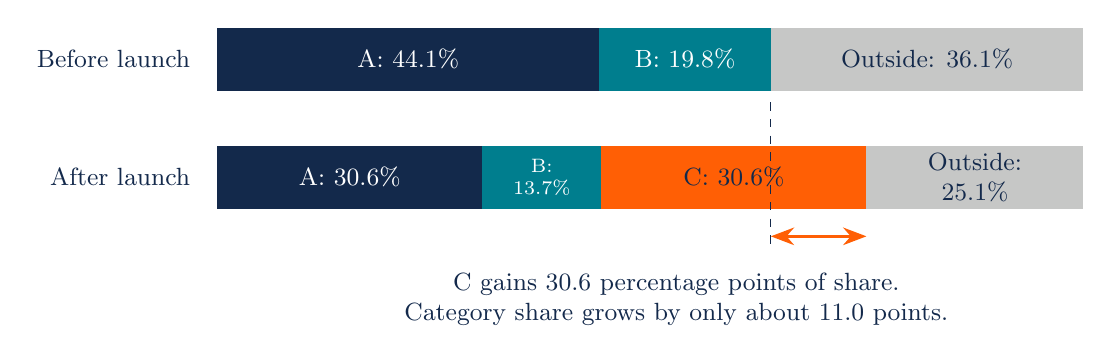
\begin{tikzpicture}[x=11cm,y=1cm]
\node[anchor=east] at (-.02,1.5) {Before launch};
\node[anchor=east] at (-.02,0) {After launch};
\fill[IlliniBlue] (0,1.1) rectangle (.4409,1.9);
\fill[Patina] (.4409,1.1) rectangle (.639,1.9);
\fill[LightStorm] (.639,1.1) rectangle (1,1.9);
\node[text=white] at (.22045,1.5) {A: 44.1\%};
\node[text=white] at (.54,1.5) {B: 19.8\%};
\node at (.8195,1.5) {Outside: 36.1\%};
\fill[IlliniBlue] (0,-.4) rectangle (.306, .4);
\fill[Patina] (.306,-.4) rectangle (.443483,.4);
\fill[IlliniOrange] (.443483,-.4) rectangle (.749475,.4);
\fill[LightStorm] (.749475,-.4) rectangle (1,.4);
\node[text=white] at (.153,0) {A: 30.6\%};
\node[text=white,font=\scriptsize,align=center] at (.3747,0) {B:\\13.7\%};
\node[text=IlliniBlue] at (.5965,0) {C: 30.6\%};
\node[align=center] at (.87475,0) {Outside:\\25.1\%};
\draw[IlliniBlue,dashed] (.639,.95)--(.639,-.85);
\draw[<->,very thick,IlliniOrange] (.639,-.75)--(.749475,-.75);
\node[align=center] at (.53,-1.55) {C gains 30.6 percentage points of share.\\Category share grows by only about 11.0 points.};
\end{tikzpicture}

\end{adjustbox}
\endgroup
\par\medskip
{\small Synthetic logit model. New bundle C has A's modeled attributes.\par}
\note{The difference between C share and incremental category demand is substitution from existing products. The logit specification makes C draw proportionally from all existing alternatives.

M4, Section 4.3, Marketing Analytics Lecture Notes. \url{../06_Lecture_Notes/modules/M04_Conjoint_Segmentation_and_CLV.md}}
\end{frame}
\begin{frame}{Incremental Contribution}
\usebeamercolor[fg]{normal text}
\vfill
\begin{slidebullets}
\item Attach contribution margins to each simulated purchase.
\item Compare the full product portfolio before and after launch.
\item Deduct development and operating costs separately.
\end{slidebullets}
\vfill
\note{Under the supplied margins of 4 dollars for A and C and 3 for B, expected contribution per potential customer rises from about 2.36 to 2.86 dollars before fixed costs. These are model-based values under imposed inputs.

M4, Section 4.3, Marketing Analytics Lecture Notes. \url{../06_Lecture_Notes/modules/M04_Conjoint_Segmentation_and_CLV.md}}
\end{frame}
\begin{frame}[fragile]{A Probability Check}
\usebeamercolor[fg]{normal text}
\noindent Calculate the synthetic baseline shares.
\begin{lstlisting}
from math import exp
utilities = {'A': 0.2, 'B': -0.6, 'Outside': 0.0}
weights = {k: exp(v) for k,v in utilities.items()}
shares = {k: v/sum(weights.values())
          for k,v in weights.items()}
assert abs(sum(shares.values()) - 1) < 1e-12
\end{lstlisting}
{\small A has about 44.1\% share, B 19.8\%, and the outside option 36.1\%.\par}
\note{For very large utilities, subtracting the maximum utility before exponentiation improves numerical stability without changing probabilities.

M4, Section 4.3, Marketing Analytics Lecture Notes. \url{../06_Lecture_Notes/modules/M04_Conjoint_Segmentation_and_CLV.md}}
\end{frame}
\begin{frame}{Substitution Assumptions}
\usebeamercolor[fg]{normal text}
\vfill
\begin{slidebullets}
\item A close copy can draw mostly from its nearest competitor.
\item Basic logit instead preserves relative odds among existing alternatives.
\item Holdout choice tasks can reveal systematic substitution errors.
\end{slidebullets}
\vfill
\note{Nested and mixed logit models relax substitution patterns under additional structure. More flexible models still need suitable choice variation and validation.

M4, Section 4.2, Marketing Analytics Lecture Notes. \url{../06_Lecture_Notes/modules/M04_Conjoint_Segmentation_and_CLV.md}}
\end{frame}
\begin{frame}{Coding Exercise: A Product Launch}
\usebeamercolor[fg]{normal text}
\vfill
\begin{slidebullets}
\item Add C to the synthetic profile table.
\item Calculate portfolio share and contribution before and after launch.
\item Compare C's share with the change in category participation.
\item Check a case with no outside option.
\end{slidebullets}
\vfill
\note{Use ../03\_Data\_and\_Code/Lecture\_Examples/session\_examples.py S05. With no outside option, purchase incidence is one by construction. That change should be visible in the program and interpretation.

M4, Section 4.10, Marketing Analytics Lecture Notes. \url{../06_Lecture_Notes/modules/M04_Conjoint_Segmentation_and_CLV.md}}
\end{frame}
\begin{frame}{Validation and Market Transfer}
\usebeamercolor[fg]{normal text}
\vfill
\begin{slidebullets}
\item Hold out respondents or tasks according to the intended use.
\item Check coding, price units, and probabilities.
\item Relate stated preference to awareness, distribution, and availability.
\end{slidebullets}
\vfill
\note{A survey share is conditional on the experiment. Real demand also depends on who sees the offering and whether they can buy it. The demand forecast needs an explicit transfer assumption.

M4, Section 4.4, Marketing Analytics Lecture Notes. \url{../06_Lecture_Notes/modules/M04_Conjoint_Segmentation_and_CLV.md}}
\end{frame}
\begin{frame}{mHealth Product Economics}
\usebeamercolor[fg]{normal text}
\vfill
\begin{slidebullets}
\item Food logs reveal recorded use and category histories.
\item A paid-plan choice model needs additional price and preference evidence.
\item Financial scenarios can state the missing inputs explicitly.
\end{slidebullets}
\vfill
\note{The lecture notes use an imposed paid-plan logit example separately from observed logs. Behavioral logging segments do not establish willingness to pay or paid subscription retention.

M4, Section 4.11, Marketing Analytics Lecture Notes. \url{../06_Lecture_Notes/modules/M04_Conjoint_Segmentation_and_CLV.md}}
\end{frame}
\begin{frame}{AI-Assisted Conjoint Analysis}
\usebeamercolor[fg]{normal text}
\vfill
\begin{slidebullets}
\item Provide the choice-set identifier and the selected alternative.
\item Require probabilities to sum to one within each task.
\item Preserve respondent groups in validation.
\item Request a portfolio comparison with explicit margins.
\end{slidebullets}
\vfill
\note{A code generator may accidentally normalize probabilities over the full dataset or treat repeated tasks as independent respondents. Small constructed tasks expose those errors.

M4, Section 4.10, Marketing Analytics Lecture Notes. \url{../06_Lecture_Notes/modules/M04_Conjoint_Segmentation_and_CLV.md}}
\end{frame}
\begin{frame}{Price Presentation and Customer Understanding}
\usebeamercolor[fg]{normal text}
\vfill
\begin{slidebullets}
\item A base price and a mandatory fee determine the total paid.
\item A stated-choice task can reveal different responses to equivalent totals.
\item The feasible pricing design depends on the applicable rule and industry.
\end{slidebullets}
\vfill
\note{The FTC's fee rule addresses live-event tickets and short-term lodging. Its scope should remain explicit. A response difference to fee framing does not itself authorize a particular presentation.

FTC Rule on Unfair or Deceptive Fees FAQ. \url{https://www.ftc.gov/business-guidance/resources/rule-unfair-or-deceptive-fees-frequently-asked-questions}}
\end{frame}
\begin{frame}{Product-Design Discussion}
\usebeamercolor[fg]{normal text}
\vfill
\begin{slidebullets}
\item How much of C's demand comes from existing products?
\item Which design change would identify the price tradeoff?
\item What evidence could change the launch recommendation?
\end{slidebullets}
\vfill
\note{The recommendation depends on substitution, incremental contribution, and costs. An appealing new-product share can coexist with little category expansion.

M4, Section 4.3, Marketing Analytics Lecture Notes. \url{../06_Lecture_Notes/modules/M04_Conjoint_Segmentation_and_CLV.md}}
\end{frame}
\end{document}
